\documentclass{article}
\usepackage{graphicx} % Required for inserting images
\usepackage{outlines}
\usepackage{svg, pdfpages}
\usepackage{wrapfig}
\usepackage{tikz}
\usepackage{url}

%\usepackage[margin=1in]{geometry}
\usepackage{enumitem}
\usepackage{boldline}
\usepackage{parskip}
\setlength{\parindent}{0em}


%Here is an updated draft project proposal incorporating the MOU between SAHA and TMM as well as the medication budget for the NCD outreach campaign:

%Title: Improving NCD Care Delivery in Somaliland through Outreach and OpenEMR

%\title{NCD Campaign in Somaliland \\
%Taiwan Medical Mission (Project)}
%\author{Dr. Tex Li-Hsing Chi}
%\date{\today}

\begin{document}


\begin{titlepage}
%    \centering

%\begin{center}
\hspace*{-0.7cm}%
\begin{tikzpicture} % tikzfigure
%\begin{minipage}[b]{1\linewidth}

\includesvg[height=3.0cm, distort=false]{Flag_of_the_Republic_of_China.svg}
\hspace{1.4cm}
%\includesvg[width=0.17\linewidth]{TMM_logo.svg}
%\hspace{3cm}
\includesvg[height=3.0cm, distort=false]{Flag_of_Somaliland.svg}
%\captionof{Figure}{xx}
%\end{minipage}
\end{tikzpicture}
    \vspace{2cm}
    
\centering
    {\Huge\bfseries Taiwan---Somaliland Flagship Project:\\
Saving My Mother, One Screening at a Time \\
- WHO Cervical Cancer Elimination Day of Action \\
    %Pap Smear Campaign, and \\
    %Cervical Cancer Screening \\
    %Training Program
    \par } % \\
 %   Handbook\par}
    \vspace{1.5cm}
    %\hspace{4cm} 
    {\Large April 2024 - November 2024 \par}

%\end{center}

\vspace{1.5cm}
%\includesvg[height=3.5cm, distort=false]{TMWH_logo(noWord).svg}
%\includesvg[height=3.0cm, distort=false]{WHD2023.svg}
\includesvg[height=3.5cm, distort=false]{anti_CervicalCancer_logo.svg}

\vspace{0.5cm}

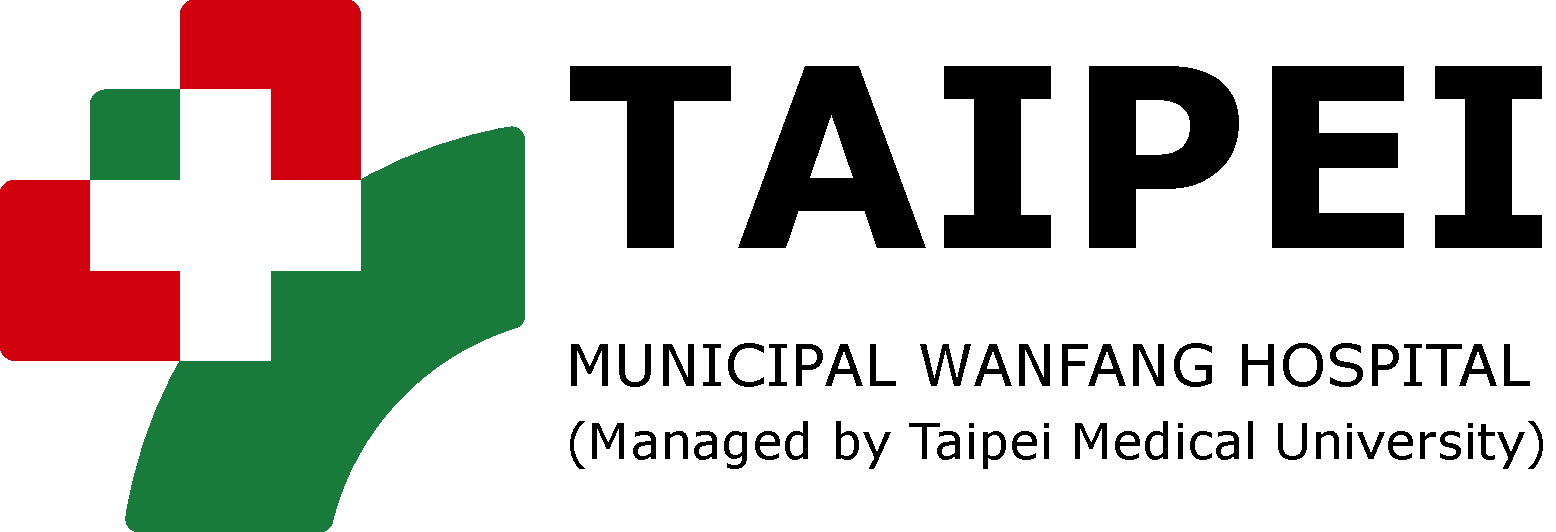
\includegraphics[height=1.9cm]{TMWH_logo_TAIPEI_vector.pdf}
\includesvg[height=2.0cm, distort=false]{logo_MoHD_HGH.svg}

%\includesvg[height=2.2cm, distort=false]{HGH_orthopedic_logo.svg}
%\includesvg[height=1.8cm, distort=false]{SAHA_logo.svg} 
%\includesvg[height=2.2cm, distort=false]{HGH_neurosurgery_logo.svg} 


%\vspace{1cm}


\end{titlepage}

%%%
%\title{Cervical Cancer Screening Training Program and Pap Smear Campaign at Hargeisa Group Hospital}
%\author{Taiwan Medical Mission}
%\date{December 2023 - January 2024}
%%%

%\hfill
%\begin{wrapfigure}[1]{l}{0.0\linewidth}%{height=0.65\textheight}
%    \centering
%    \includesvg[width=0.20\textwidth]{TMM_logo.svg}
%\end{wrapfigure}
%\vspace{1.5cm}

%\maketitle

\noindent
\begin{minipage}{0.2\textwidth}
\centering
\includesvg[width=0.9\linewidth]{TMM_logo.svg}
\end{minipage}
\hfill
\begin{minipage}{0.75\textwidth}
\centering
{\LARGE\bfseries TMM---HGH \\ 
Pap Smear Campaign and \\
Pathology Training Program }\\[1ex]
\large\textit{Dr. Tex Li-Hsing Chi}\\[2ex]
\today
\end{minipage}


%%%
\section{Background}
Taiwan Medical Mission (TMM) aims to build medical capacity in the Republic of Somaliland through specialty training exchanges, outreach programs, and visiting scholar opportunities at Hargeisa Group Hospital (HGH).
% , and developing equipment maintenance capabilities

TMM has announced a Pap smear campaign, telepathology, and outreach campaigns by visiting specialists.
TMM is also establishing a visiting scholar program for HGH staff to train in Taiwan.

Key initiatives planned for 2023-2024 are:

\begin{itemize}
\item Hemodialysis - AV fistula surgery training, tele-nephrology conferences
%\item Critical care - local and Taiwan ICU training
\item Orthopedics - local and Taiwan orthopedic surgeon training
\item NCD clinic - partnership with NGO SAHA on NCD prevention
\item Nursing fundamentals training program
\item Visiting specialists - Taiwanese specialists performing surgeries and training
\item Telepathology for case discussions and virtual consults
%\item Teleradiology and telepathology platforms
\item Outreach campaigns on Pap smear, orthopedic/trauma, oral health, blood donation, and osteoporosis awareness
\item Visiting scholar program for HGH staff to train in Taiwan (since 2023)
%\item Procurement of medical equipment and maintenance training
\end{itemize}

%To support these initiatives, TMM has proposed a 
%budget of around USD 442,000 for 2024. This includes funding for relief supplies, visiting scholar program, equipment, transportation, and program activities.
% , upgrade equipment and maintenance capabilities,

%The goal is to exchange specialty knowledge, expand access to care, and improve public health outreach. This will build local capacity at HGH through collaboration between Somaliland and Taiwanese healthcare professionals.




\section{Introduction}
%Cervical cancer remains one of the top causes of cancer deaths among women in Somaliland, with mortality rates estimated to be over 20 per 100,000, more than 4 times higher than Taiwan. 

Cervical cancer is a preventable and curable disease, yet it remains the 4th most common form of cancer among women worldwide. 
Despite having successfully implemented a national cervical cancer screening program since 1995 in Taiwan that has reduced incidence and mortality by over 70\%, screening coverage in Somaliland remains extremely low, well under 5\%.
Barriers to screening include limited medical infrastructure and personnel, low awareness among women, and sociocultural taboos. Our Taiwan Medical Mission team has been collaborating with Hargeisa Group Hospital since July 2023 to establish cervical cytology capacity. With enormous effort, we have set up Somaliland's first Pap smear screening clinic in HGH. However, much work remains to expand services, train local staff, and educate women to utilize screening.
To accelerate progress in saving women's lives, we propose a concentrated one-month training program and screening campaign since April 2024. Renowned OB/GYN doctors from Taiwan will provide hands-on instruction in specimen collection and developing streamlined screening protocols. Leading pathologist Dr. Chang will conduct intensive Pap stain, cytology, and pathology workshops to increase the quality and efficiency of interpretation. 

%This project seeks to expand screening and treatment capacity for all women ages 21-65 at risk of cervical abnormalities.
% https://www.cdc.gov/cancer/cervical/basic_info/screening.htm

The Taiwan Medical Mission proposes a medical campaign called "WHO Cervical Cancer Elimination Day of Action" to launch an awareness drive across Hargeisa to motivate women to get screened from April 2024 to November 2024. Our hashtags are \#GlowTeal and \#CervicalCancer.

%
The Cervical Cancer Elimination Day of Action is an annual event that takes place on November 17th. It marks the anniversary of the launch of the "Global Strategy to Accelerate the Elimination of Cervical Cancer" as a public health problem by the World Health Organization (WHO).
In May 2018, the WHO Director-General announced a global call for action to eliminate cervical cancer, underscoring renewed political will to make elimination a reality and calling for all stakeholders to unite behind this common goal. In August 2020, the World Health Assembly adopted the Global Strategy for cervical cancer elimination. Now is the time to act to eliminate cervical cancer as a public health problem.


%

Cervical cancer screening can help detect abnormal cells in the cervix before they develop into cancer. The two main types of cervical cancer screening tests are the Human papillomavirus (HPV) DNA test and the Pap test.
Human papillomavirus (HPV) is a commonly transmitted infection that can cause 70\% of cervical cancer in women. HPV infection often has no symptoms, so many people may not know they have it. There are many different types of HPV, some of which can cause cancer.
An HPV DNA test can identify high-risk HPV varieties (i.e., 16 and 18) that are most likely to cause cervical cancer.
These tests are advised for women aged 30 to 49, with regular testing every 5–10 years.
During a Pap test, a sample of cells from the cervix is obtained and analyzed for abnormalities by a cytologist.
Moreover, WHO has renewed its recommendations for screening and treatment of cervical cancer, making clear that HPV DNA-based tests are more efficient than cytology-based tests (i.e., Pap test), especially for low- and middle-income countries, because they are less prone to quality problems (WHO 2021: \Url{https://www.who.int/europe/news/item/11-09-2021-who-recommends-dna-testing-as-a-first-choice-screening-method-for-cervical-cancer-prevention}).


If abnormal cells or HPV infection are detected during cervical cancer screening, further testing and treatment may be necessary. Treatment options for pre-cancerous lesions include biopsy, cryosurgery, laser surgery, loop electrosurgical excision procedure (LEEP), cold knife conization, and abdominal total hysterectomy (ATH). These treatments aim to remove abnormal cells, which will be investigated by a pathologist for diagnosis and safety margin of tumor.

We will propose using the "screen-triage-treat" approach via HPV DNA testing, which has been recognized by the WHO as the primary screening method for eliminating cervical cancer globally.
We plan to build referral networks for precancer treatment and cancer care.
This project will also enable the HPV self-sampling initiative, a widely used HPV testing method, to discover best practices in low-resource service delivery.


%%% why breast cancer screening
Breast cancer is also among the most common and fatal cancers affecting women globally. According to WHO, breast cancer accounts for nearly 12\% of all new annual cancer cases and is the second leading cause of cancer death among women. In low and middle-income African countries, outcomes are worse due to more advanced staging at diagnosis and lack of adequate screening programs and cancer therapy resources. 

Breast cancer screening in Taiwan has evolved over the past two decades. Mammography screening is recommended for average-risk women ages 45-69 every 2 years. In 2002, Taiwan launched a nationwide breast cancer screening program providing biennial mammography for women 45-69 along with clinical breast exams.


Implementing mammogram screening for women during the target cervical cancer screening age range can enable early breast cancer detection in an efficient and cost-effective manner. Managing any detected abnormalities or positive cancer diagnoses would be facilitated through support from the visiting TMM general surgeon during his time onsite in 2024. Overall, adding mammography and breast cancer diagnosis/treatment components serves to make the service model even more comprehensive and impactful for this population.


%%%%
\section{Aim}

Improve early detection and management of cervical precancer/cancer in Somaliland by expanding screening coverage and treatment access. This aligns with WHO’s vision for attaining the highest possible level of sexual and reproductive health worldwide, in which cervical cancer is an eliminable disease.
As per WHO's Global Strategy adopted in 2020, this project aims to accelerate Somaliland’s progress towards the 2030 targets of 90\% HPV vaccination coverage, 70\% cervical cancer screening coverage, and 90\% access to pre-cancer treatment and cancer care including palliative services. 

%Our mission is aligned with WHO’s Sexual and Reproductive Health and Research (SRH) division which has driven the adoption of the cervical cancer elimination resolution and strategy. With the tools available today, eliminating cervical cancer is within reach - but only with concerted effort can these live-saving interventions reach all women in need.

%%%


\section{Objectives}

%%% *** why and rationale
The main objective of this project is to improve breast/cervical cancer prevention and screening in Somaliland by implementing the 2021 WHO recommendation guideline, which includes HPV DNA testing. (\url{https://www.who.int/europe/news/item/11-09-2021-who-recommends-dna-testing-as-a-first-choice-screening-method-for-cervical-cancer-prevention})

\begin{itemize}
\item Train at least 4 OB/GYN doctors and 10 midwives in proper HPV DNA test and Pap test procedures
\item Train at least 2 pathology technicians in Pap stain methodology
\item Train at least one pathologist doctor in cytology/pathology diagnoses
\item Train at least 2 general surgeons in breast cancer screening, diagnosis and treatment

\item Screen and provide results for 1,000+ women in Hargeisa
\item Provide HPV vaccine (one shot) for 1,000+ girls by the age of 15

\item Develop streamlined protocols for large-scale screening implementation
\item Increase public awareness and demand for breast/cervical cancer prevention
\end{itemize}


The project aims ultimately to achieve the following targets by 2030: 
\begin{outline} 
\1 Vaccination: 90\% of girls fully vaccinated with the HPV vaccine by the age of 15. 
\1 Screening: 70\% of women screened using a high-performance test, including HPV DNA test, by the age of 35, and again by the age of 45. 
\1 Treatment: 90\% of women with pre-cancer treated and 90\% of women with invasive cancer managed.
\end{outline}


%
\section{Methods}
\begin{itemize}

\item[] \textbf{TMM Visiting Specialists}
Comprehensive Cervical Cancer Control (CCCC) seeks to expand screening and treatment support for women at risk of cervical abnormalities. 
Gynecologist Dr. Chun-Sen Hsu and Dr. Yu-Hsin Huang from Taiwan will collaborate with Dr. Fatima, Director of OB/GYN at Hargeisa Group Hospital, from April-September 2024.
They will provide specialized gynecologic care, perform additional cervical cancer screening via HPV/Pap testing, conduct workshops on navigating cervical abnormalities and cancer, and develop tailored protocols for managing cervical health for Somaliland women.

General surgeon doctor from Taiwan will be onsite February-July 2024. He can assist and teach with evaluating abnormal breast imaging findings, performing ultrasounds and biopsies for suspicious lesions, advising on breast cancer treatment options, and providing minor surgical procedures if feasible. Coordinating mammogram screening during his visit will enable diagnostic workup and treatment connections for any detected breast abnormalities or cancers.

\item[]\textbf{Training Activities}
% Describe training workshops, screening drive, awareness campaign, etc.

\begin{itemize}
\item Hands-on HPV DNA and Pap smear workshops for OB/GYN and midwives
\item Pap stain methodology sessions for pathology technicians
\item Cytology/pathology sessions for pathologist doctors
\item Lectures on international best practices and quality assurance
\item Joint discussions to develop standardized protocols for cervical cancer (and breast cancer) screening, diagnosis, and treatment

\end{itemize}

%%%%
\item[]\textbf{Screening Campaign}


The campaign will implement several strategies to improve cervical cancer prevention and screening in Somaliland: 

\begin{outline} 
\1 In-person communication and information material at Hargeisa Group Hospital (HGH): This can include brochures, posters, A5-sized notes from the hospital information system (HIS) at OPD, and other informational materials that explain the importance of breast/cervical cancer screening, how to get screened with ultrasound, mammogram, HPV DNA test, and Pap smear, and the benefits of vaccination against HPV. 
\1 Media promotions through TV, radio, posters, and social media
\1 Better recall through SMS (Telesom or Somtel) written in Somali languages: A system (a.k.a. \textbf{PathoPush}) can be set up to send reminders to women through SMS. These reminders can include information about how to attend a screening, recall for further therapy in case of abnormal findings of HPV DNA test or Pap smear, and when their next screening is due.
\1 Incentives: People can be encouraged to attend screenings through free health checks, small gifts (like multivitamin tablets), recognition, or small rewards. 
\1 Offering breast ultrasound, mammogram and cervical cancer screening together during a screening campaign can provide women with the opportunity to have two important health screenings at the same time. 
\1 Verbal communication through seminars and workshops: Seminars and workshops can be organized to educate women about their risk of cancer and the importance of screening. 
\1 Screening approaches:
    \2 screen-treat method: Taking HPV DNA and Pap smear, then follow or treat according to cytology result by PathoPush system
    \2 screen-triage-treat (mobileODT) at once: It offers a full turnkey diagnostic and treatment program utilizing the HPV DNA rapid test, the EVAPro digital colposcope, and loop electrosurgical excision procedure (LEEP)/conization (or thermocoagulation, ThermoGlide) treatment of precancerous lesions
\1 Connect cancer-diagnosed patients to available treatment options (referral for breast cancer and cervical cancer)
\1 Provide incentives support for Somaliland local medical team involved in breast/cervical cancer prevention workflow
\end{outline}

%
\begin{itemize}
\item Media promotions through TV, radio, posters, hospital bus, and social media
%\item Patient navigator support and follow-up system
\item Streamlined workflow to maximize patients screened
\item Streamlined protocols for processing specimens, patient tracking, results notification, and follow-up
\item Data collection on screening statistics and outcomes (openEMR system)
\item Scientific publication
\item Policy suggestion for Ministry of Health Development (MoHD)
\end{itemize}

\end{itemize}
%%%%

\section{Sustainability} 
To ensure the sustainability of the project, several measures will be implemented: 

\begin{outline} 
\1 Collaboration with local organizations: Partnering with local organizations can help to ensure that the campaign is culturally sensitive and tailored to the needs of the local population. 
\1 Training of healthcare professionals: Training healthcare professionals on the importance of cervical cancer screening and how to perform HPV DNA tests and Pap smears can help to ensure that women receive high-quality care. 
\1 Regular follow-up: Regular follow-up with women who have attended screenings can help to ensure that they receive appropriate care if any abnormalities are detected. 
\1 Data collection and analysis: Collecting data on the number of women who attend screenings, the results of their tests, and any follow-up care they receive can help to evaluate the effectiveness of the campaign and identify areas for improvement. 
\1 Funding: Securing long-term funding for the campaign from organizations such as WHO, Prevent Cancer Foundation, or European Society for Medical Oncology (ESMO) can help to ensure its sustainability. 

\end{outline}

%%%%

%\section{Activities}

%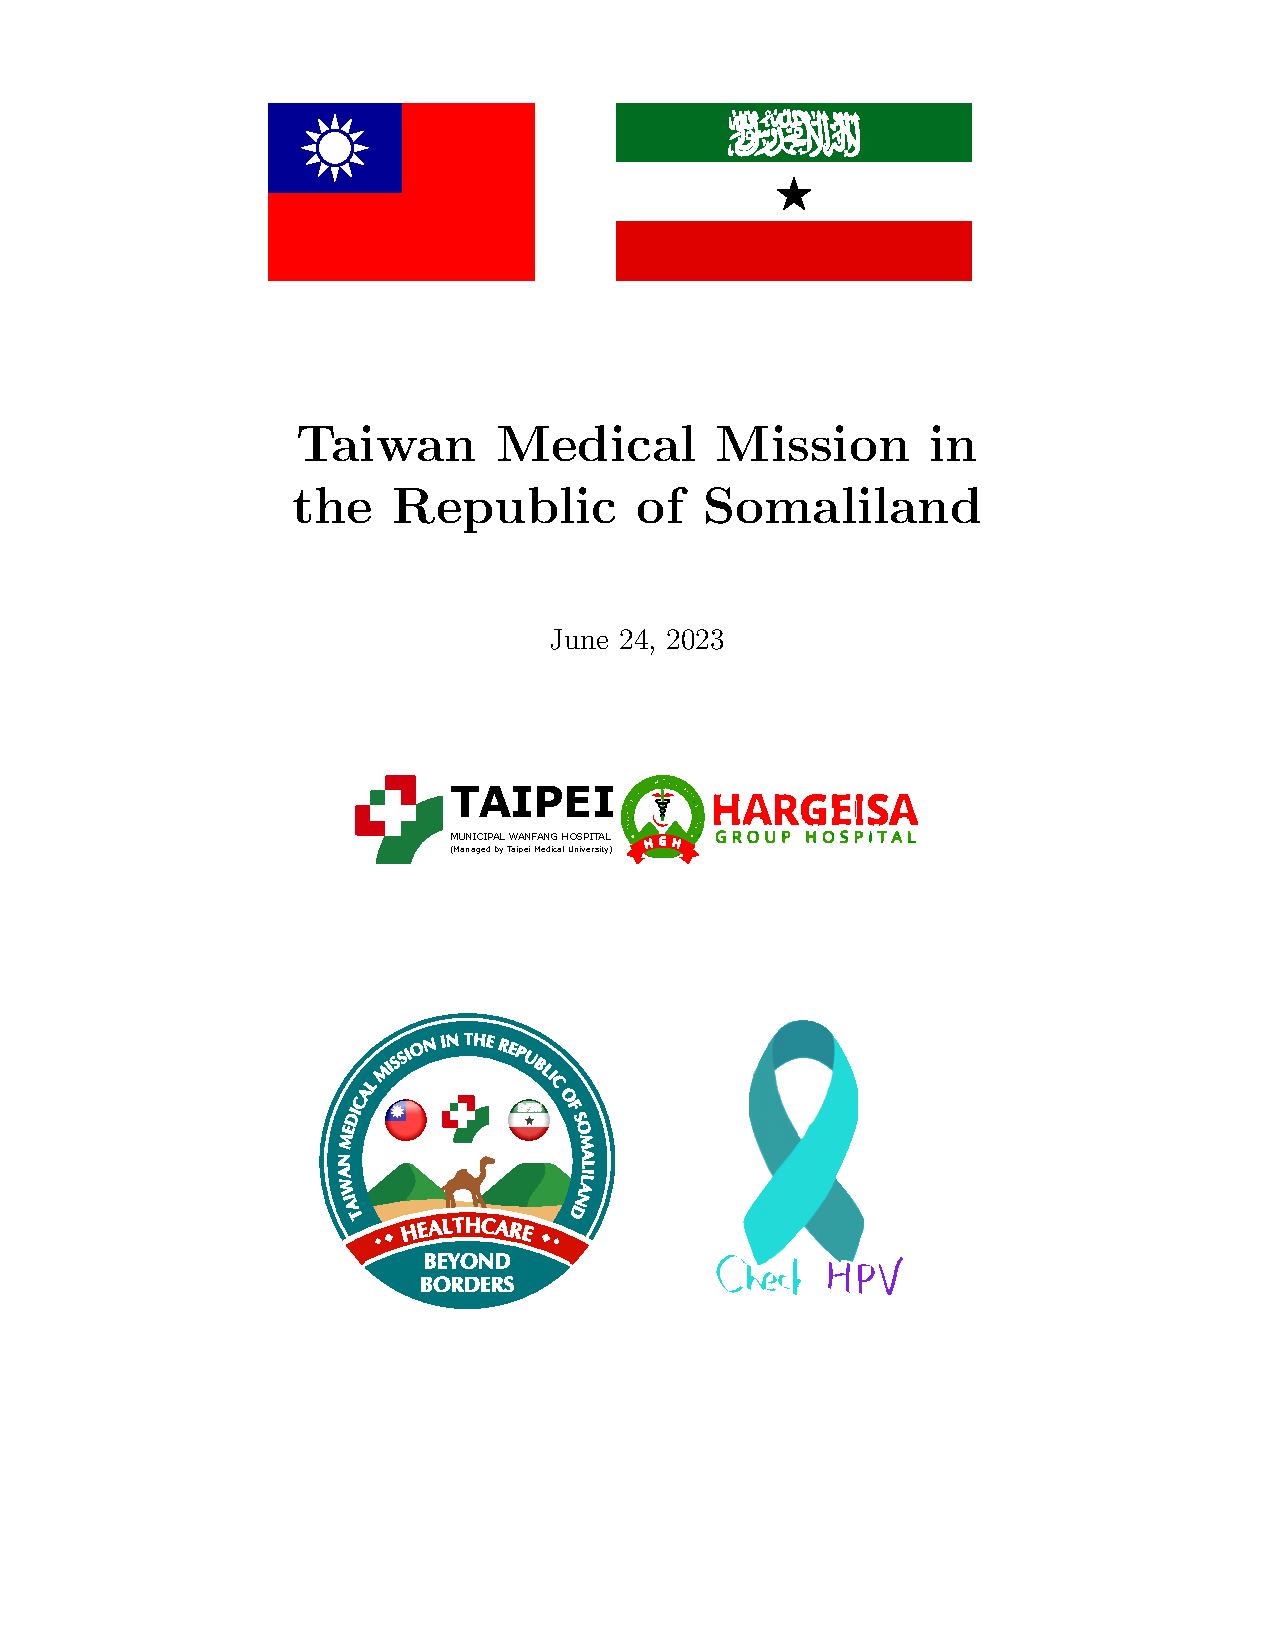
\includepdf[pages=-]{TMM_SLN_20231117_WorldCervicalCancerEliminationDay_WCCED_project__.pdf}
\clearpage



%%%

\section{Expected Outcomes}
% Quantify expected training numbers, screening numbers, other impacts
The expected outcomes of this project include: 
\begin{outline} 

\1 Increased awareness and participation in breast/cervical cancer prevention among women in Somaliland:
    \2 Screen and provide results for 1,000+ women in Hargeisa
    \2 Provide HPV vaccine (one shot) for 1,000+ girls by the age of 15

    \2 Increased diagnosis and treatment of precancerous cervical lesions and breast cancer
\1 Improved access to high-quality breast/cervical cancer prevention services for women in Somaliland:
    \2 Enhanced local capacity in managing breast/cervical abnormalities and cancer
    \2 Train at least 4 OB/GYN doctors and 10 midwives in proper HPV DNA and Pap test procedures
    \2 Train at least 2 pathology technicians in Pap stain methodology
    \2 Train at least 2 general surgeons in breast cancer diagnosis and treatment
    \2 Develop streamlined protocols for large-scale screening implementation
    \2 Implement PathoPush and openEMR system for documentation and reporting purposes
    \2 Self-sustaining breast/cervical prevention program with motivated screening team
\end{outline}


%%%%%%%%%%%%%%

%\section{Challenges}
% Discuss potential challenges and limitations


%%%%%%%%%%%%%%%%%

\section{Challenges and Solutions}
With strong collaboration, planning, and adaptable implementation, the challenges can be overcome to make the initiatives successful.

\begin{outline}

%\1 Limited surgical equipment and supplies
%\2 Partner with TMM for procurement of essential tools, implants, consumables

%\1 Infrastructure limitations in OT
%\2 Optimize existing infrastructure, explore facility upgrades

%\1 Shortage of trained surgical staff
%\2 Hands-on training by Dr. Kuo, virtual learning, visiting scholar program

%\1 Referral delays for complex cases
%\2 Streamline referral process, utilize telemedicine for prompt consultations

\1 Limited public awareness of women's health
\2 Engaging outreach with clear educational messaging

\1 Transportation barriers for patients
\2 Arrange logistics support for those in need

%\1 Post-op care coordination
%\2 Cross-training nurses, protocols to facilitate care transitions

%\1 Data limitations for monitoring
%\2 Implement tracking logs to collect key metrics

\end{outline}




\section{Conclusion}
%Wrap up with importance of this effort to save women's lives
The primary objective of this project is to enhance the effectiveness of breast/cervical cancer prevention and screening efforts in Somaliland through the use of evidence-based tactics and the utilization of bioinformatics science. These approaches will be specifically customized to address the unique requirements and characteristics of the local population.


By successfully attaining its stated goals, this program has the potential to make a significant contribution towards the eradication of cervical cancer as a prevailing public health concern in Somaliland. The implementation of this pathology training program has the potential to enhance the cancer diagnostic capabilities of Hargeisa Group Hospital, positioning it as a leading healthcare center in the Horn of African countries.


\clearpage




%%
\clearpage

% April - September 2024 Dr. Huang

\section{(draft) Budget Planning}
Costs to include:
\begin{outline}
\1 Screening tools

\2 Pap smear instruments, materials, and cytology/pathology reagents (to be delivered at HGH in July 2023)
\2 HPV DNA test instrument and kits
\2 Diagnostic mammography x-ray machine, ultrasound for breast/pelvic examinations
\2 Immunohistochemistry (IHC) staining process (sending to Ethiopian pathology laboratory)
\2 RadiPush and PathoPush systems (Telesom's SMS enabled) and openEMR system (open-sourced software) with laptop computers
\2 Incentives for the medical practitioners and technicians contributing to the Pap smear/Pap stain workflow

\1 Diagnosis tools

\2 Colposcopy with camera
\2 Cryosurgery equipment
\2 LEEP/conization electrodes and unit
\2 Breast surgical instruments for biopsy and minor procedures

\1 Printed educational booklet with Somali language translation
\1 "Saving My Mother, One Screening at a Time" - WHO Cervical Cancer Elimination Day of Action (Ceremony on 2024/11/17)


%\1 Bone density screening machine
\end{outline}

%Total: USD 10,000


\section{Supplement Material}
A draft presentation/booklet Cervical Cancer Awareness and Prevention: (coming soon)

%\documentclass{beamer}
\usepackage{graphicx}

\title{Trauma Awareness and Injury Prevention \\
- For World Trauma Day}
\author{Dr. Tex Li-Hsing Chi}
\date{17th Octocber 2023}

\begin{document}

\begin{frame}
\titlepage
\end{frame}

\begin{frame}
\frametitle{Trauma Burden}
\begin{itemize}
\item Trauma is a major cause of death and disability worldwide. Over 310,000 pedestrians were killed in crashes 2016, accounting for 23\% of all global deaths.
\item The proportion of pedestrians killed compared with other road users is highest in the WHO African Region, at 40\%, and lowest in the WHO South-East Asian Region at 14\%.
\item At least 50\% of road accident deaths in developing countries are preventable
\item In Somaliland, road traffic accidents and falls are common causes of injury  
\end{itemize}
\end{frame}

\begin{frame}
\frametitle{Awareness Saves Lives}
\begin{itemize}
\item Recognize signs of serious injury - bleeding, fractures, head injury
\item Call for help immediately - alert medical providers
\item Initiate first aid if trained - stop bleeding, immobilize fractures
\item Transport safely - avoid further harm enroute 
\end{itemize}  
\end{frame}

\begin{frame}
\frametitle{Injury Prevention}
\begin{itemize}
\item Safe driving - avoid distractions, enforce speed limits, add speed humps/bumps to slow traffic in busy pedestrian areas
\item Seat belts and child safety seats  
\item Protective gear - helmets, guards, harnesses 
\item Safe work practices - proper training, supervision
\item Home and public safety - handrails, window guards 
\end{itemize}
\end{frame}

\begin{frame}
\frametitle{WHO Pedestrain Safety}
    \begin{itemize}
        \item Key points adopted from the WHO Pedestrian Safety manual to highlight for preventing pedestrian injuries in Hargeisa:
        \begin{itemize}
            %\item 
            \item Separating pedestrians from vehicles - Sidewalks, barriers, to reduce interaction
            \item Improving visibility - Lighting, reflective paint, so drivers see pedestrians
            \item Education campaigns - Teach pedestrian and road safety skills, rights and responsibilities
            \item Law enforcement - Ensure drivers yield to pedestrians, stop at crossings, obey signals and speed limits
            \item Data collection - Gather injury data to identify problem areas and infrastructure needs
        \end{itemize}

%Planning and legislation - Develop master plans and policies to integrate pedestrian safety
    \end{itemize}
\end{frame}

\begin{frame}
\frametitle{First Aid Saves Lives}
\begin{itemize}
\item Learn first aid skills - take a course
\item Assess for dangers first
\item Control bleeding with direct pressure  
\item Immobilize fractures with splints
\item Monitor head injuries closely 
\end{itemize}
\end{frame}

\clearpage

\begin{frame}
\frametitle{Trauma Care}
\begin{itemize}
\item Timely treatment is critical - "golden hour"
\item Stabilize patient and address immediate threats
\item Imaging helps guide interventions - x-ray, CT
\item Multidisciplinary approach by doctors, nurses, therapists
\end{itemize}  
\end{frame}

\end{document}

%Let me know if you would like me to modify the content or format of the presentation in any way. I'm happy to add more details on specific injury prevention methods or treatment approaches.

%%
\section{Acknowledgment}
We would like to express our gratitude to the medical practitioners and personnel at the HGH and TMWH facilities, specifically those working in the departments of Obstetrics and Gynecology, as well as Pathology.


%\section{Reference}
%(1) Interpreting the Lancet surgical indicators in Somaliland: a cross-sectional study. https://bmjopen.bmj.com/content/10/12/e042968 Accessed 11/05/2023.
%(2) ENT Department | Somali Sudanese specialized hospital. ENT Department | Somali Sudanese specialized hospital (ssshospital.so) Accessed 11/05/2023.


\end{document}
